\section{Measurement and Analysis}
\subsection{Motivating Examples}
\vspace{-0.2in}
\begin{figure}[htb]
\centering
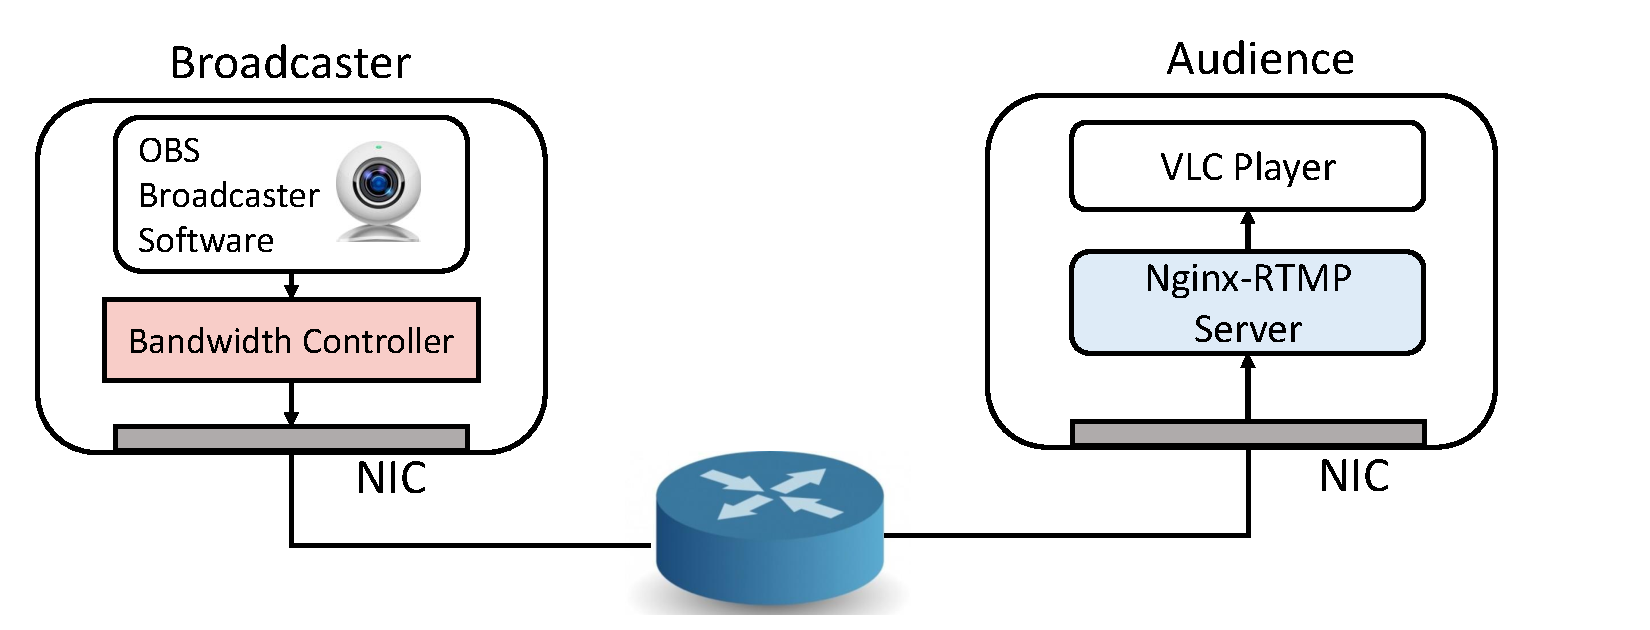
\includegraphics[width=\columnwidth]{fig/setup.pdf}
\caption{Experiment setup}
\vspace{-0.1in}
\label{fig:setup}\mylabel{fig:setup}
\end{figure} 
\textbf{Experiment setup.} We set up a live video streaming framework as in Figure~\ref{fig:setup}. The demo comprises of two modules, broadcaster and audience, which are connected by a switch in the middle. Servers both have 2 CPU cores and 6GB memory, and are equipped with $100$Mbps NICs. OBS studio\cite{OBS} is one popular broadcast software and is used to stream videos to the audience side over RTMP protocol. We use both the tc module of linux and dummynet\cite{dummynet} to control the real-time upload bandwidth of broadcaster. The receiving server is built on nginx-rtmp module. On the audience server, VLC player is used to play the rtmp streaming.

%\begin{figure}[htb]
%\centering
%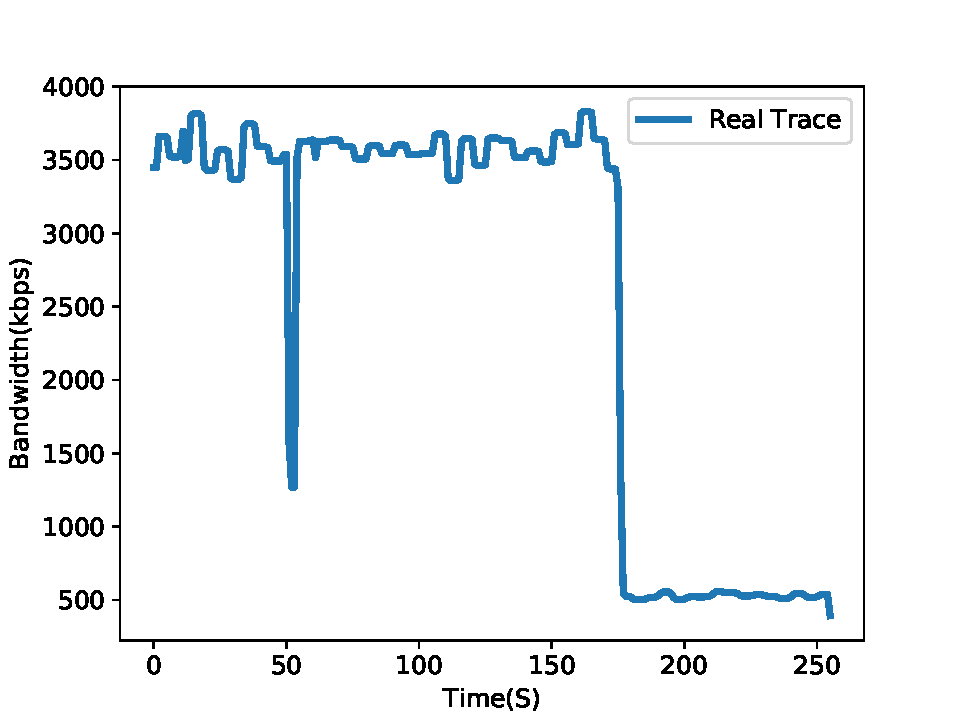
\includegraphics[width=.8\columnwidth]{fig/case_study_bandwidth.pdf}
%\caption{Bandwidth Control}
%\label{fig:case-bandwidth}\mylabel{fig:case-bandwidth}
%\end{figure}

\begin{figure}[htb]
\centering
\begin{subfigure}[b]{.45\columnwidth}
\centering
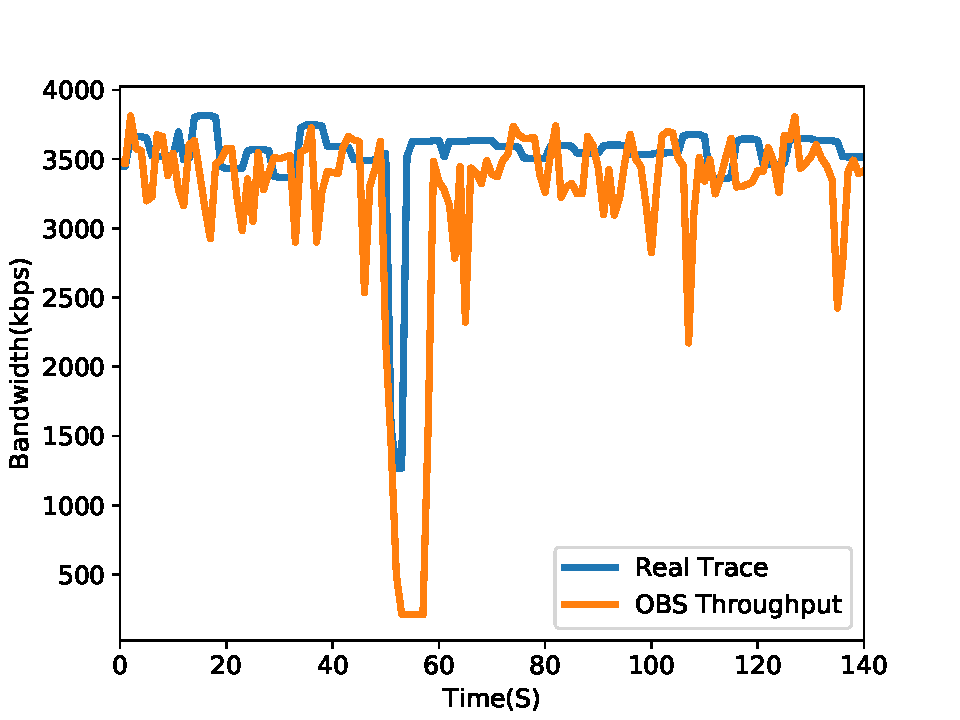
\includegraphics[width=\textwidth]{fig/case_study_throughput_a.pdf}
\caption{Throughput of $0-140$s}
\label{fig:case-throughput-a} \mylabel{fig:case-throughput-a}
\end{subfigure}
\begin{subfigure}[b]{.45\columnwidth}
\centering
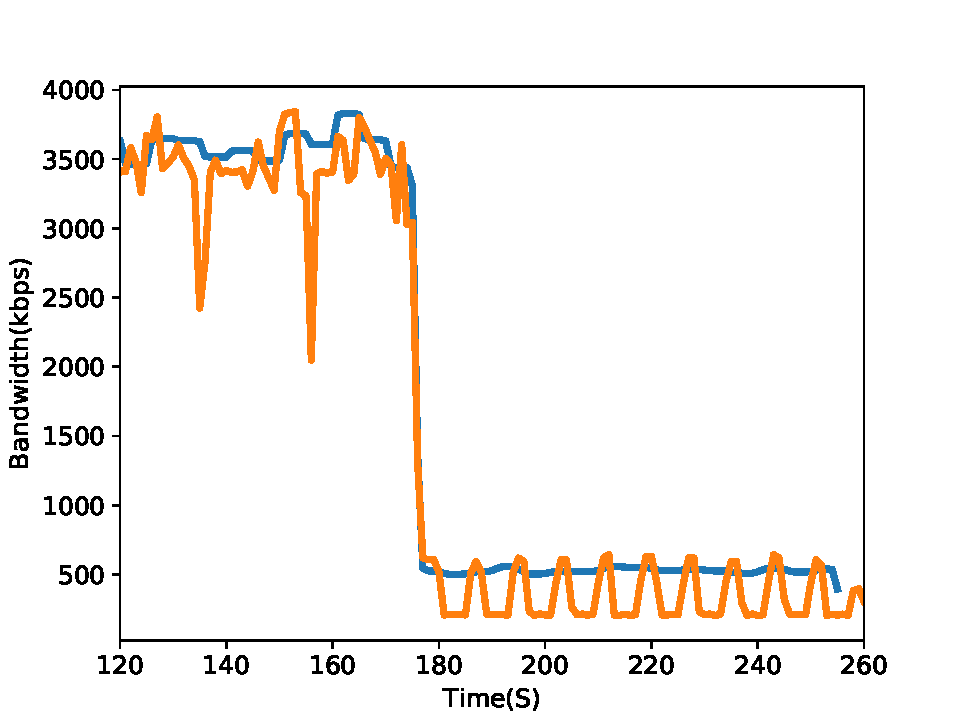
\includegraphics[width=\textwidth]{fig/case_study_throughput_b.pdf}
\caption{Throughput of $120-260$s}
\label{fig:case-throughput-b} \mylabel{fig:case-throughput-b}
\end{subfigure}
\caption{Case study: video streaming throughput in oscillating wireless network}
\label{fig:case-throughput} \mylabel{fig:case-throughput}
\end{figure} 
\textbf{Case study.} In the first motivating experiment, we control the network bandwidth according to an actual trace from a wireless network. The trace records the real-time network conditions when a user join the www.amazon.com on a mobile device. We aggregate packets in the trace into 5-second bins and calculate the data amount in each slot. We then control the network bandwidth on the broadcaster-side according to the per-second profile. The average bandwidth is up to $3000$kps, we stream video at a bitrate of $3000$kbps via OBS and capture actual video packet trace using tcpdump in the audience's side. And the result is shown in Figure~\ref{fig:case-throughput}.  The trace lasts for $320$s, such a long time that we break the trace into two parts.

In the figure~\ref{fig:case-throughput-a}, the actual throughput follows the trace closely. However, at 50s, the network bandwidth falls below the bitrate and the situation lasts for 2 seconds, while the actual throughput degrades to almost zero from 50s to 58s. This is an abnormal behavior, as \textit{a 2-second network jitter cascadingly causes 8-second throughput falling in the streaming application.} Besides, a constant bitrate cannot efficiently handle long-term the bandwidth variance, which can be seen in Figure~\ref{fig:case-throughput-b}. Bandwidth is enough during $0-180s$, but after $180s$, the available bandwidth drops dramatically and lasts for $80s$, endless frames drop in this period. In this challenging network environment, the default OBS insists previous bitrate and obviously the strategy is not enough.

\begin{figure}[htb]
\centering
\begin{subfigure}[b]{.45\columnwidth}
\centering
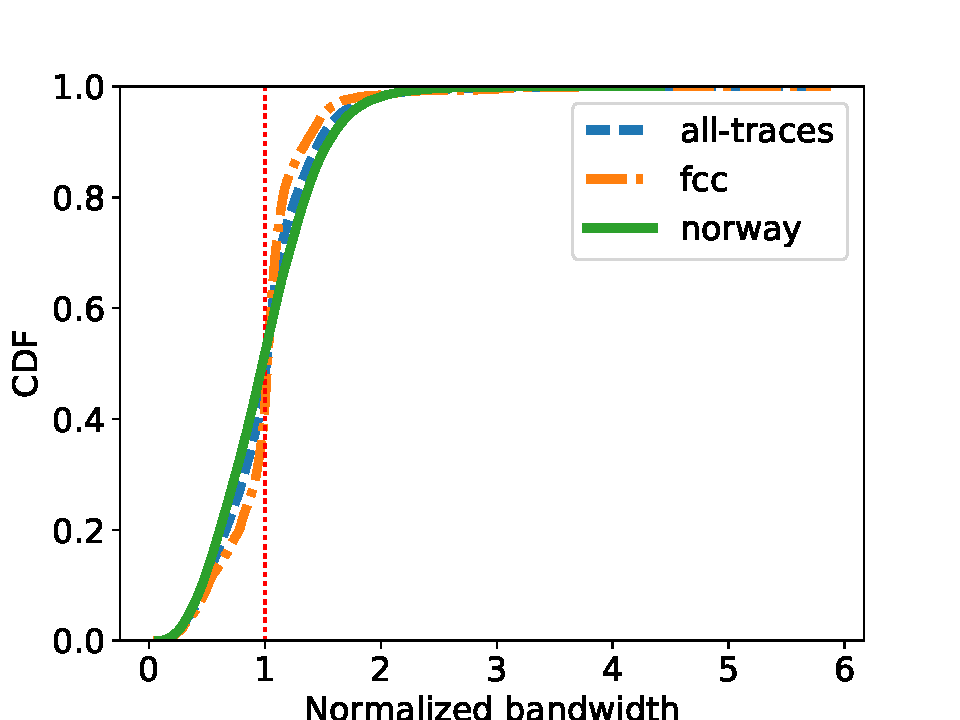
\includegraphics[width=\textwidth]{fig/trace.pdf}
\caption{Normalized Bandwidth}
\label{fig:trace}\mylabel{fig:trace}
\end{subfigure}
\begin{subfigure}[b]{.45\columnwidth}
\centering
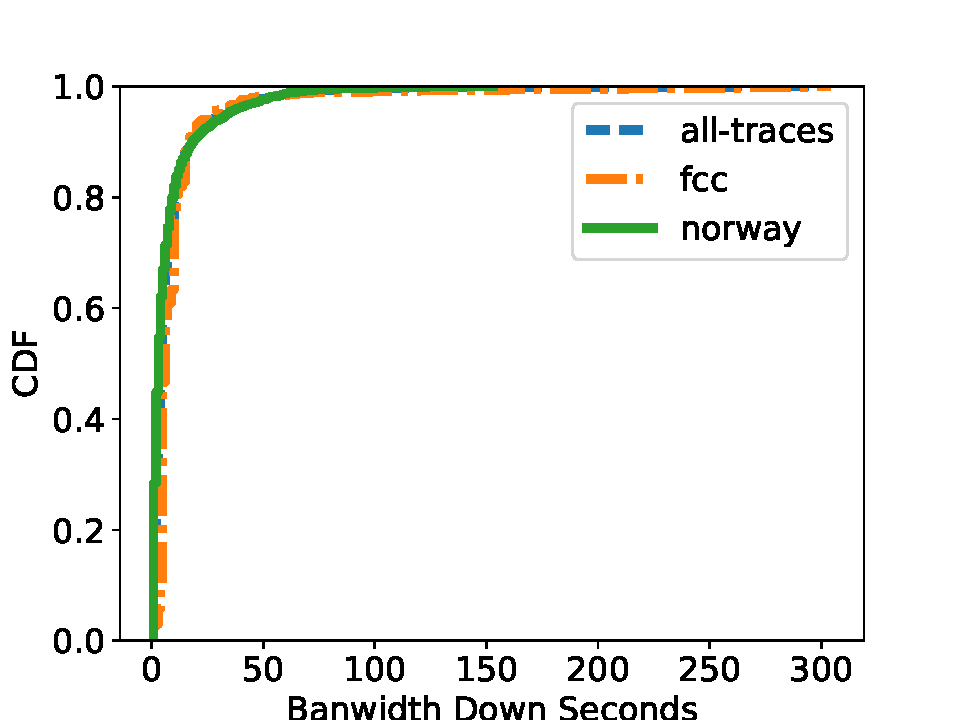
\includegraphics[width=\textwidth]{fig/trace-down.pdf}
\caption{Throughput Drop Time}
\label{fig:trace-down}\mylabel{fig:trace-down}
\end{subfigure}
\caption{Bandwidth distribution in wireless network}
\label{fig:trace-all}\mylabel{fig:trace-all}
\end{figure}

\textbf{Network Conditions.} To know how often the bandwidth failure occurs, first we want to know the bandwidth distribution of real world. Two real-world dataset, FCC dataset~\cite{FCC_dataset} and HSDPA dataset~\cite{HSDPA_dataset}, is combined to calculate the bandwidth failure ratio. Each trace lasts for 320s, and the total dataset lasts for $30$ hours. For each trace, referring the average bandwidth as the unit, we normalize the trace and draw the cdf(Figure.~\ref{fig:trace}). Almost $50\%$ of traces are under the average throughput, which means for a $10$ second trace, about $5$ second the bandwidth is lower than the average. About $20\%$ of the traces are at most half of the average. The figure indicates that in real-time network, bandwidth fluctuation frequently occurs. To further explain how often long-term bandwidth fluctuation happens, we draw a picture of network failure time distribution, Figure~\ref{fig:trace-down}. Network failure time is calculated by counting the continuing time lower than the average bandwidth. About $20\%$ of the bandwidth fluctuation lasts for more than $10$ seconds, some even lasts for hundreds of seconds. Always using constant bitrate may introduce massive frame dropping.

\begin{figure*}[htb]
\begin{subfigure}[b]{0.32\textwidth}
  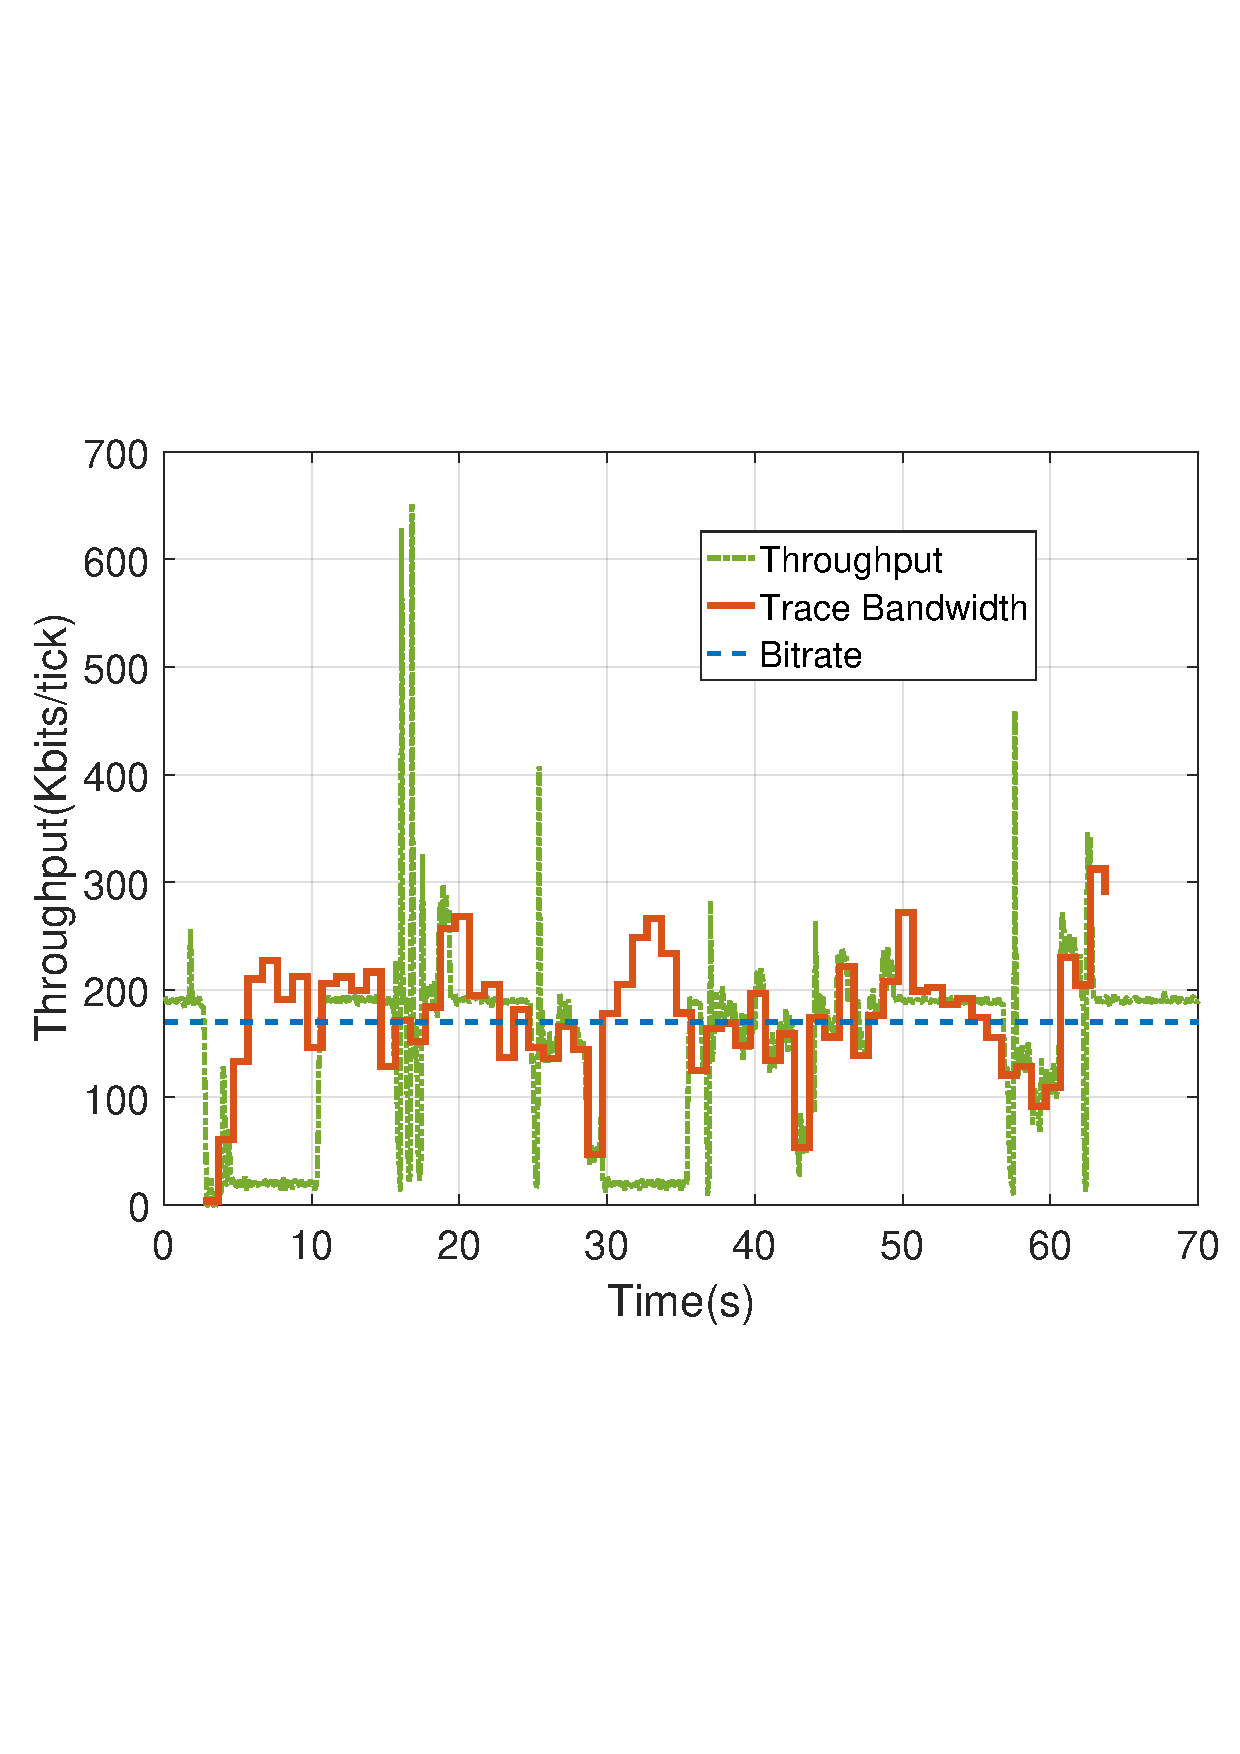
\includegraphics[width=0.8\linewidth]{fig/obs_douyu.pdf}
  \vspace{-0.05in}    
  \caption{OBS to Douyu server}
  \label{fig:obs-douyu}\mylabel{fig:obs-douyu}
\end{subfigure}
\begin{subfigure}[b]{0.32\textwidth}
  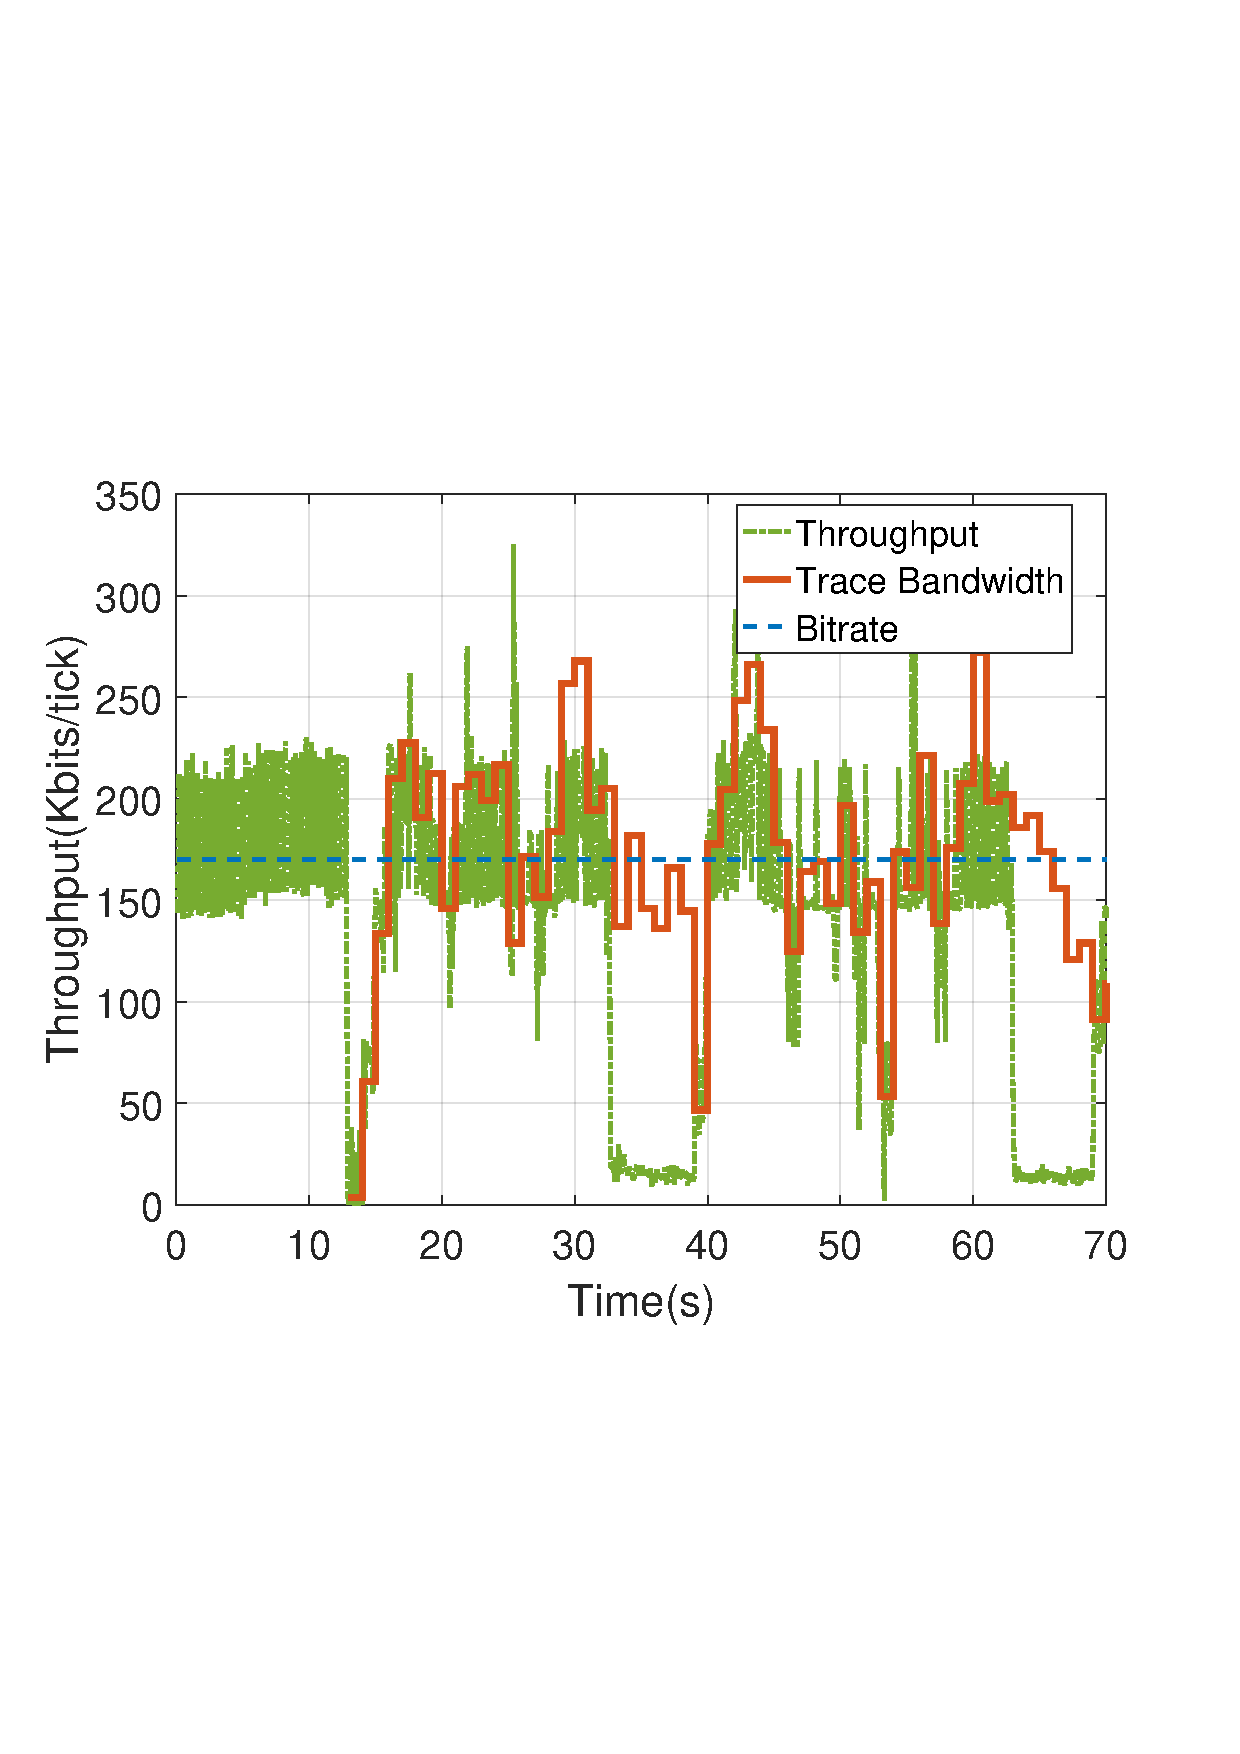
\includegraphics[width=0.8\linewidth]{fig/douyu.pdf}
  \vspace{-0.05in}    
  \caption{Douyu broadcaster to Douyu server}
  \label{fig:douyu}\mylabel{fig:douyu}
\end{subfigure}
\begin{subfigure}[b]{0.32\textwidth}%
  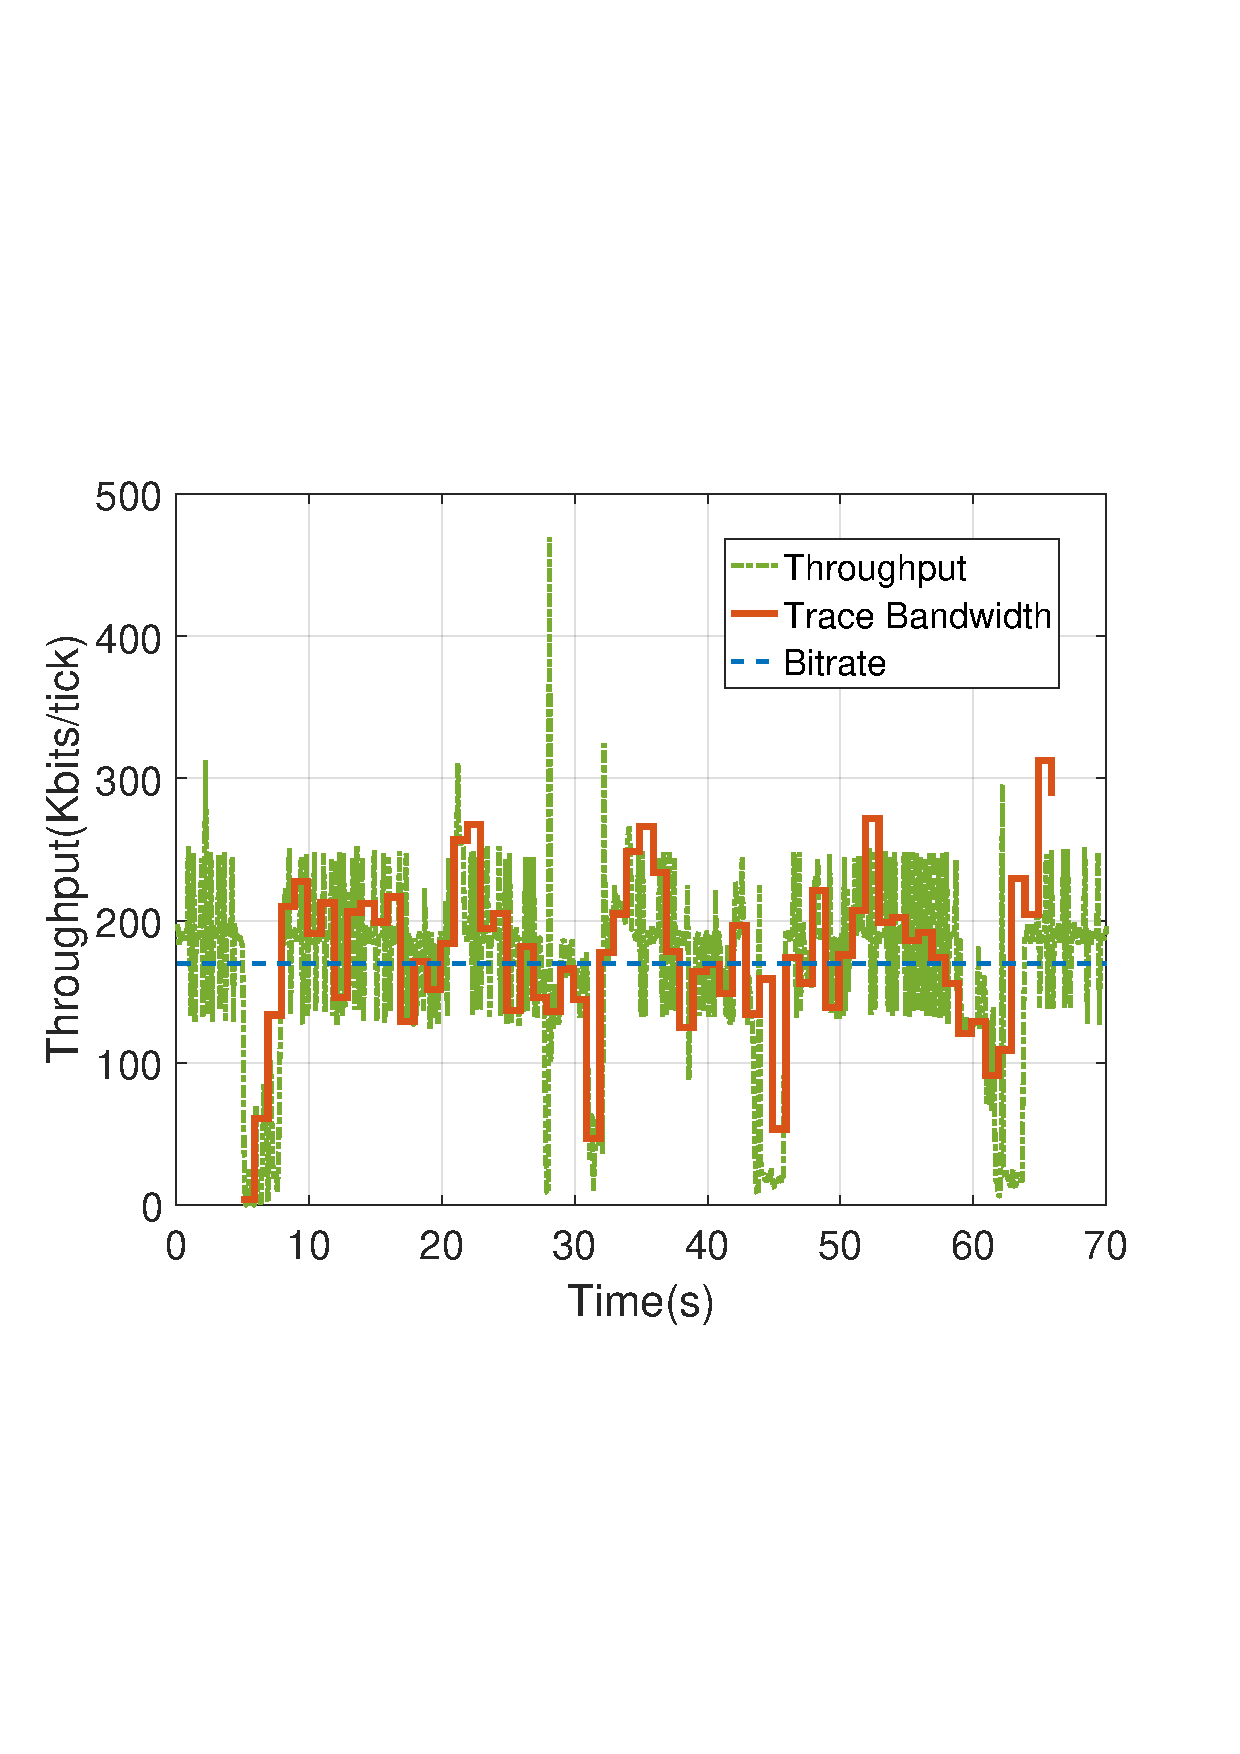
\includegraphics[width=0.8\linewidth]{fig/obs_twitch.pdf}
  \vspace{-0.05in}    
  \caption{OBS to Twitch server}
  \label{fig:obs-twitch}\mylabel{fig:obs-twitch}
\end{subfigure}
\caption{Throughput in three experiments}
\vspace{-0.15in}
\label{fig:commerical-throughput}
\end{figure*}

\begin{figure*}[htb]
\begin{subfigure}[b]{0.32\textwidth}
  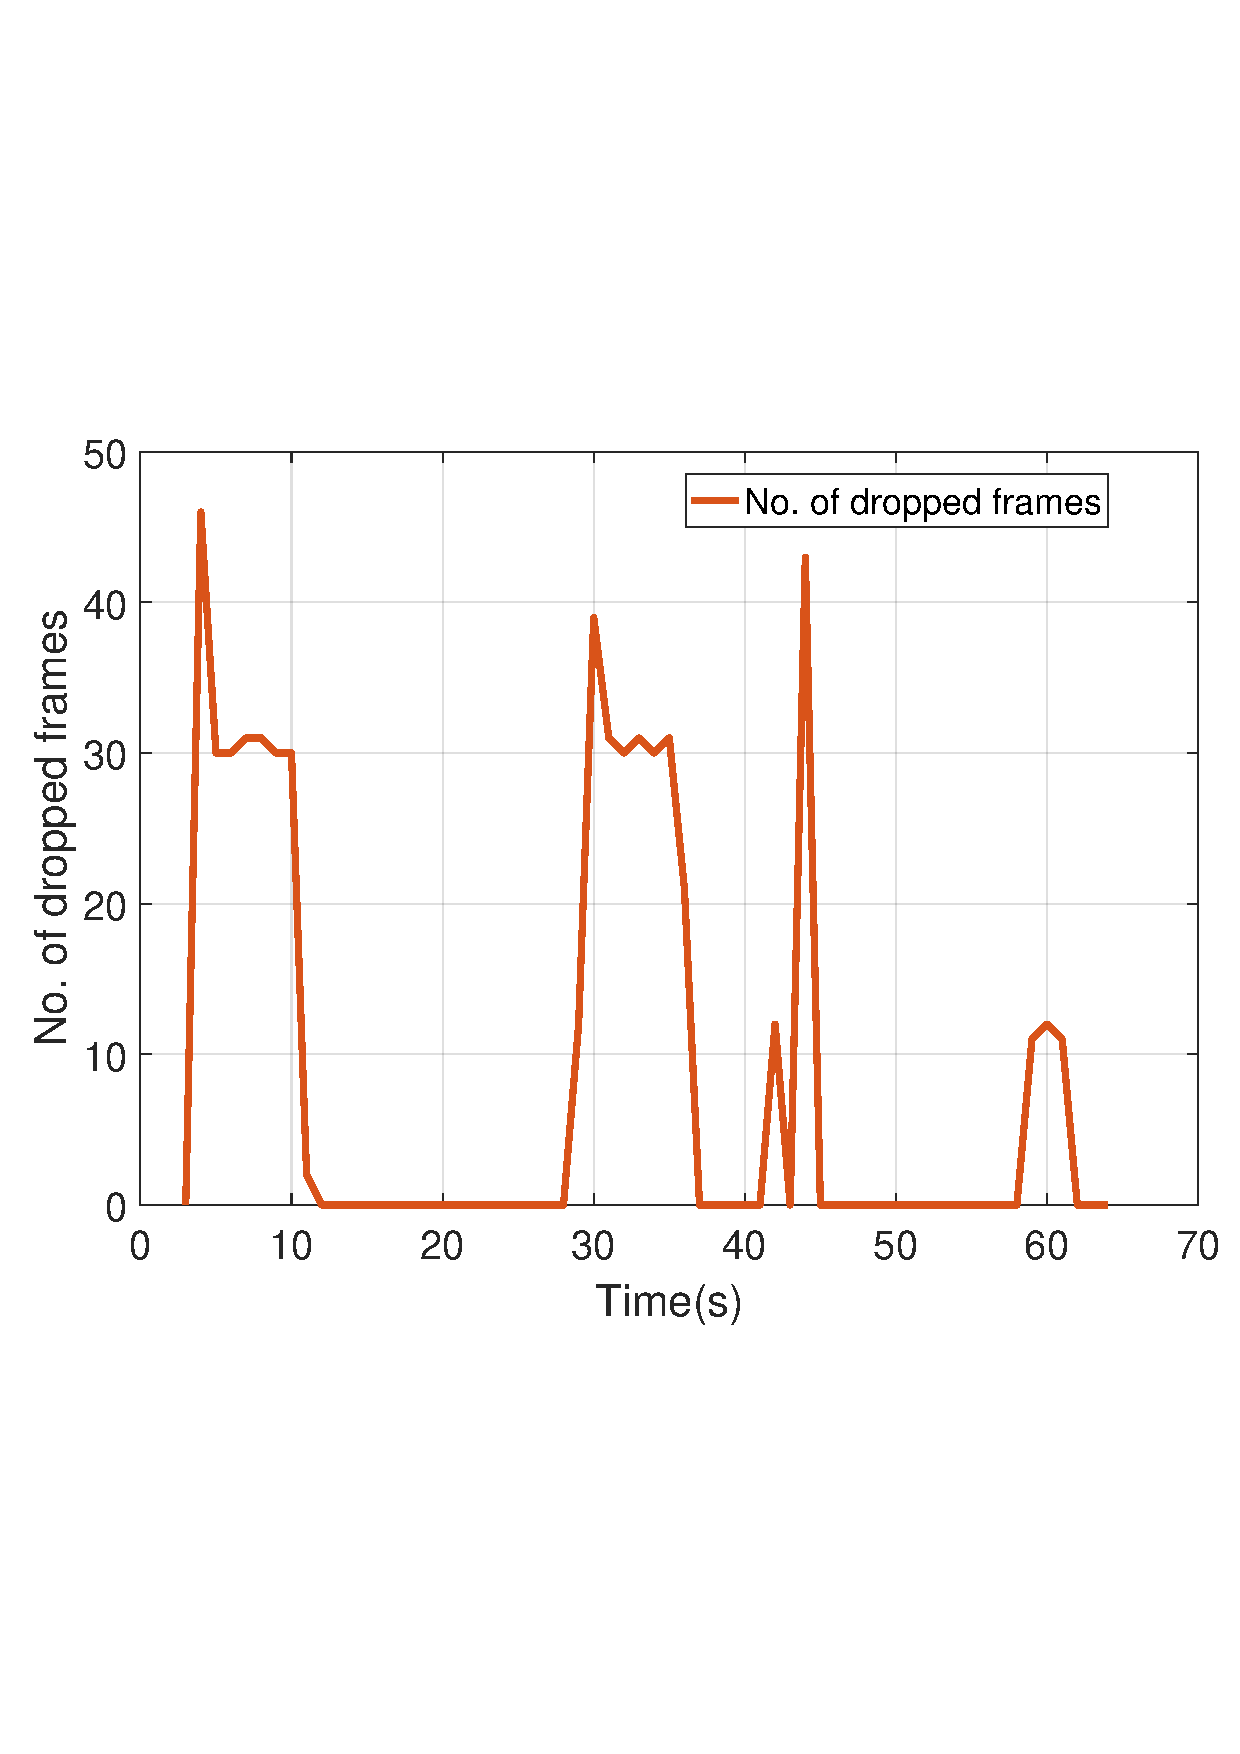
\includegraphics[width=0.8\linewidth]{fig/obs_douyu_drop.pdf}
  \vspace{-0.05in}  
  \caption{OBS to Douyu server}
  \label{fig:obs-douyu-drop}\mylabel{fig:obs-douyu-drop}
\end{subfigure}
\begin{subfigure}[b]{0.32\textwidth}
  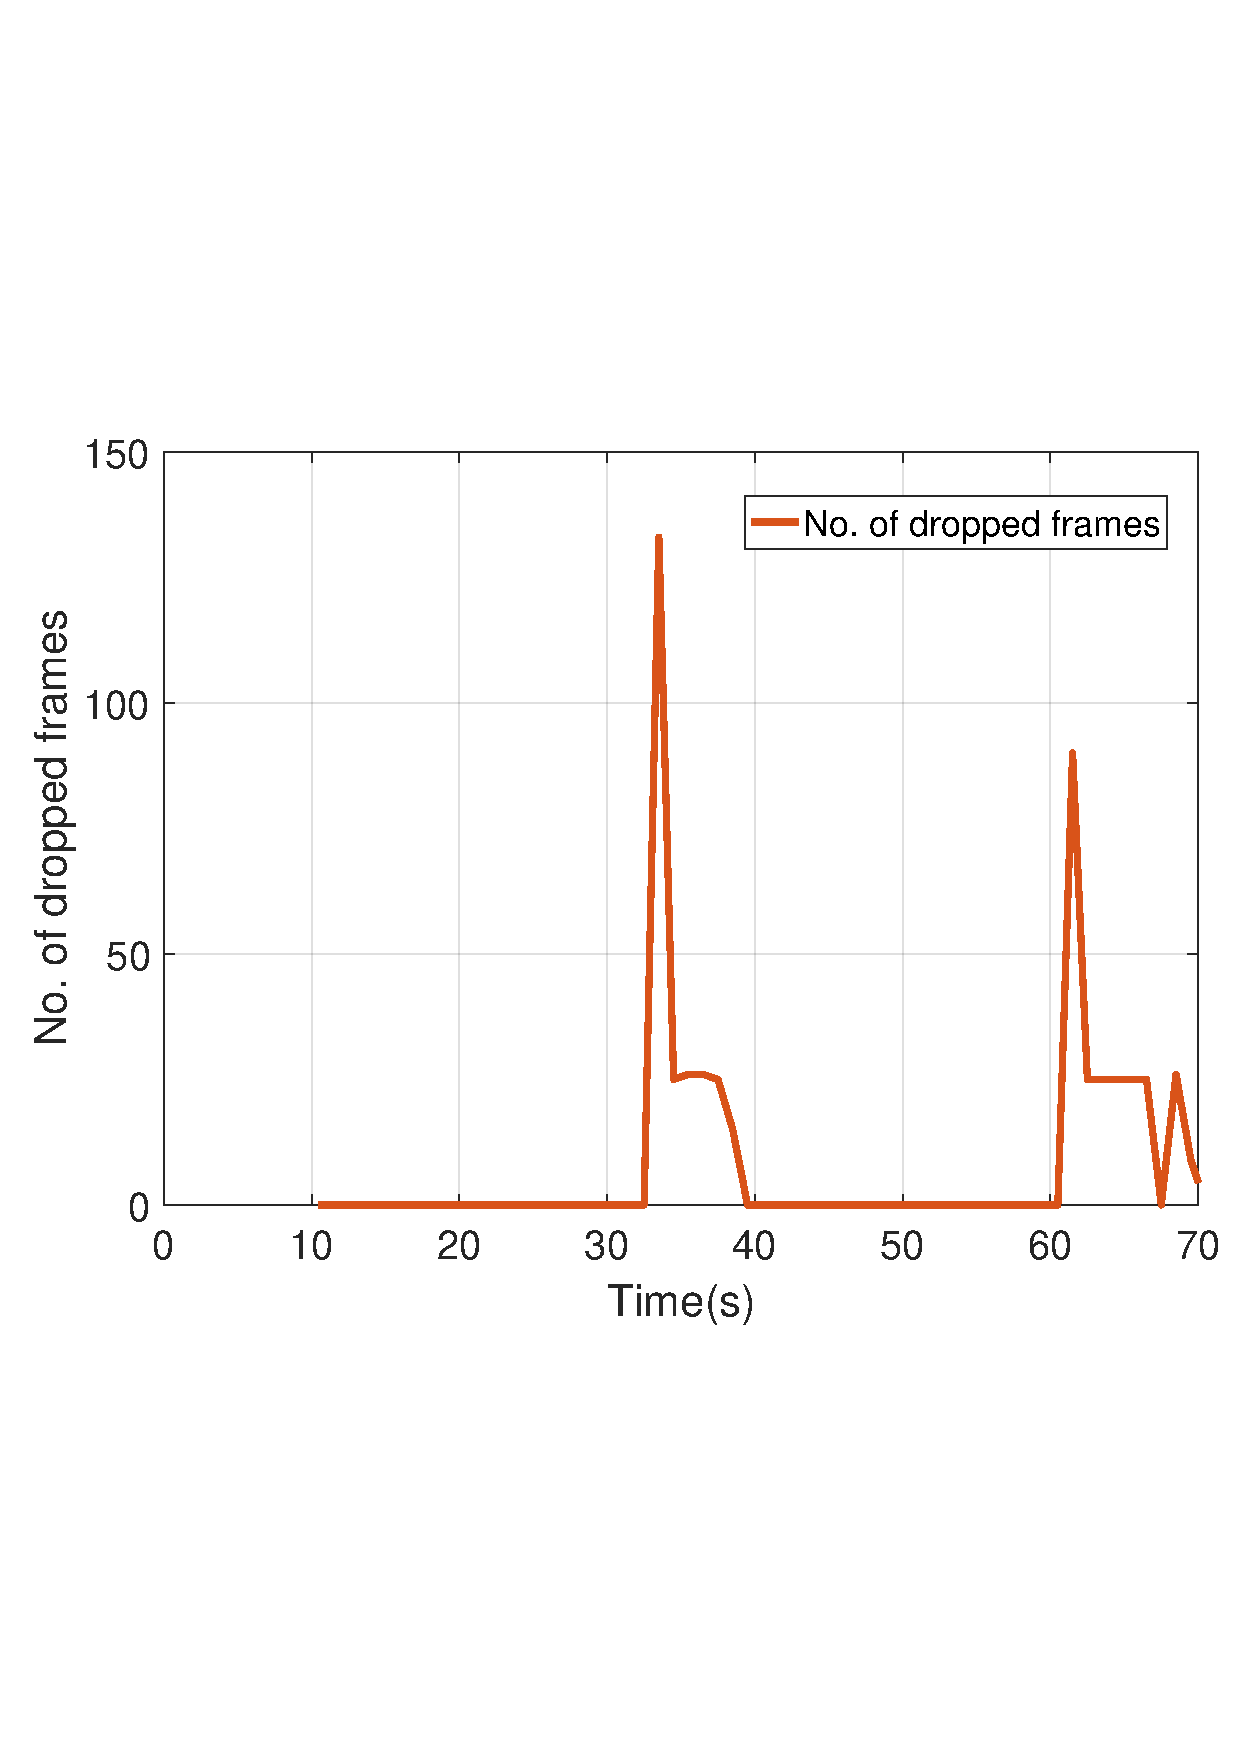
\includegraphics[width=0.8\linewidth]{fig/douyu_drop.pdf}
  \vspace{-0.05in}    
  \caption{Douyu broadcaster to Douyu server}
  \label{fig:douyu-drop}\mylabel{fig:douyu-drop}
\end{subfigure}
\begin{subfigure}[b]{0.32\textwidth}%
  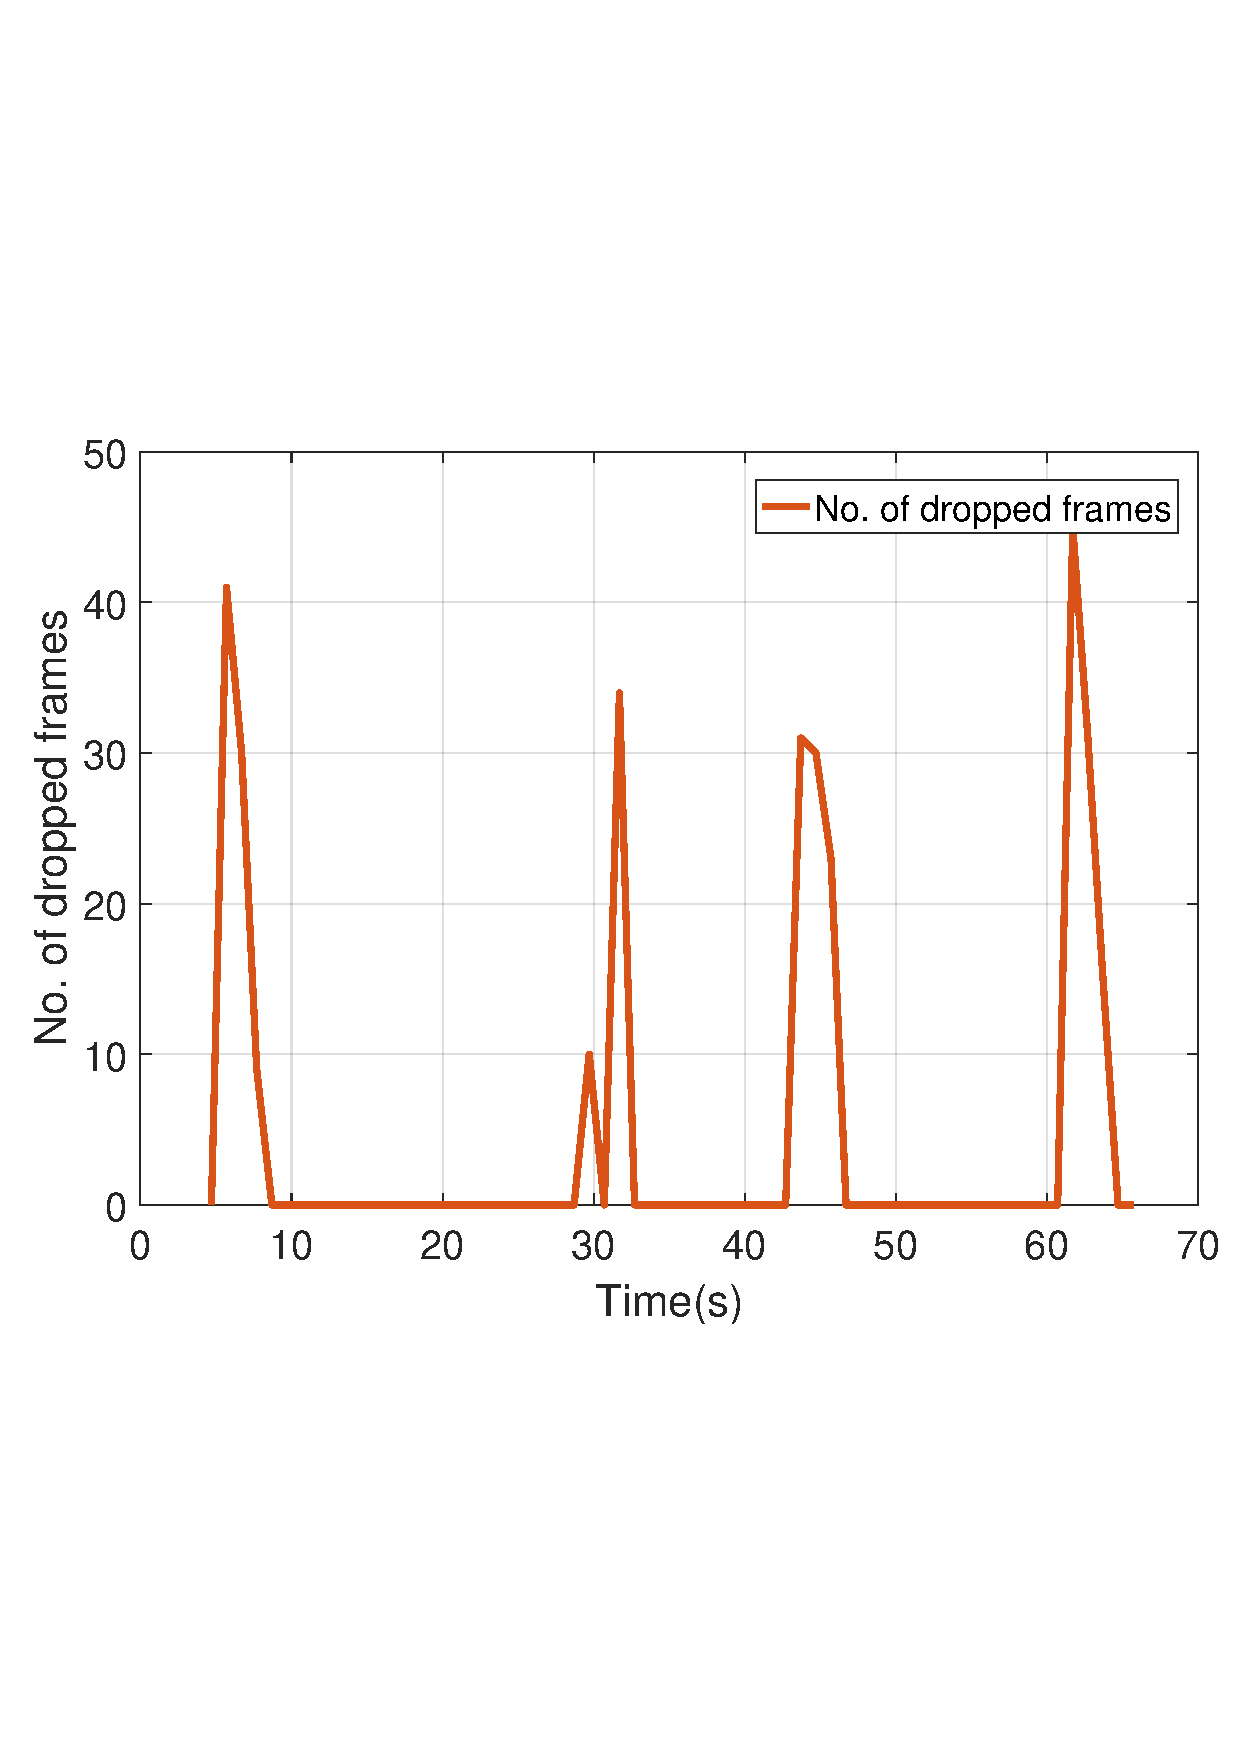
\includegraphics[width=0.8\linewidth]{fig/obs_twitch_drop.pdf}
  \vspace{-0.05in}    
  \caption{OBS to Twitch server}
  \label{fig:obs-twitch-drop}\mylabel{fig:obs-twitch-drop}
\end{subfigure}
\caption{No. of dropped frames}
\vspace{-0.2in}
\label{fig:commerical-drop}
\end{figure*}

\begin{figure}[htb]
\centering
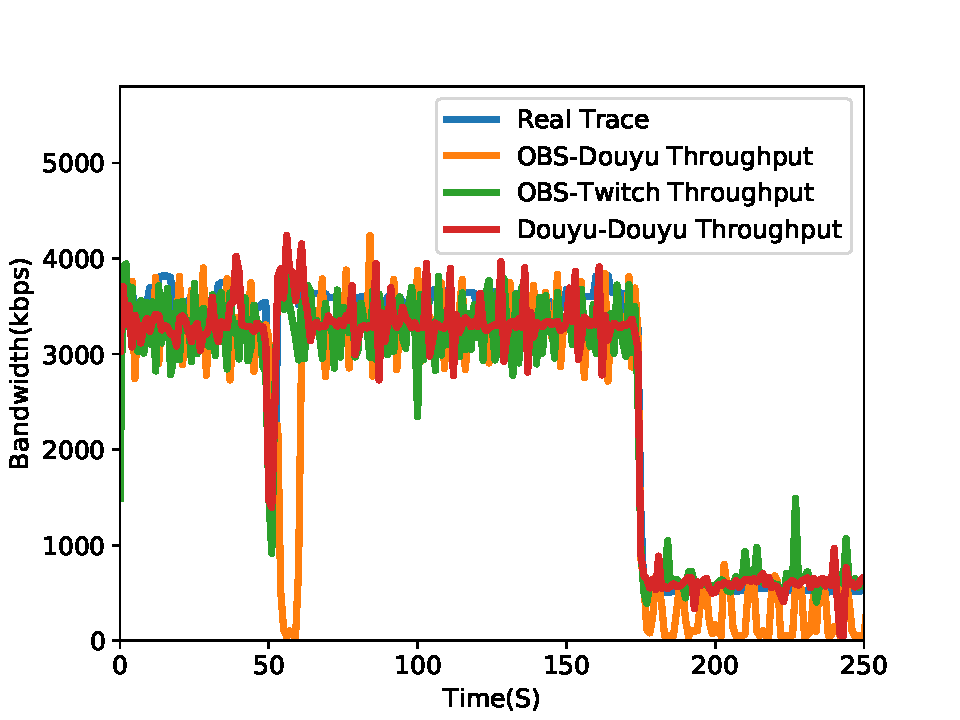
\includegraphics[width=.7\columnwidth]{fig/vary-bandwidth.pdf}
\vspace{-0.05in}
\caption{Throughput in long-time bandwidth drop case}
\vspace{-0.15in}
\label{fig:vary-bandwidth}\mylabel{fig:vary-bandwidth}
\end{figure}

\begin{table}[tb]
\centering
\caption{Frames dropped in different scenarios}
\label{tbl:drop}
{\setlength{\tabcolsep}{1pt}
\begin{tabular}{|c|c|c|l|}
\hline
\textbf{Experiment} & \textbf{Scenario} & \textbf{Play Failure(S)} & \textbf{ Failure Percentage(\%)}   \\ \hline
\multirow{3}{*}{Figure 5}&  Obs-douyu               & 18.1         & 30.2\%                           \\ \cline{2-4}
& Obs-twitch              & 9.9        & 16.3\%    \\ \cline{2-4}
& Douyu-douyu            & 16.6      & 27.2\% \\ \hline
\multirow{4}{*}{Figure 7} & Obs-douyu            & 93.1      & 37.2\%     \\ \cline{2-4}
& Obs-twich             & 79.3      & 31.7\%  \\ \cline{2-4}
& Douyu-douyu             & 66.67         & 26.7\%  \\ \hline
\end{tabular}}
\vspace{-0.2in}
\end{table} 
\textbf{Experiments on several commercial platforms.} We further repeat the experiment in different commercial platforms and settings to find whether the same issues exist. We test three different situations, including OBS pushing video to Douyu server, Douyu broadcaster to Douyu server, and OBS to twitch server. In three experiments, the bitrate is choose lower than the average bandwidth, $1700$kbps. Tcpdump is used to record the real-time throughput, we aggregate the data size in each tick(0.1s) together and draw a picture.
Figure~\ref{fig:obs-douyu}, ~\ref{fig:douyu}, and~\ref{fig:obs-twitch} show the throughput of the three experiments respectively, ~\ref{fig:obs-douyu-drop}, ~\ref{fig:douyu-drop}, ~\ref{fig:obs-twitch-drop} is the corresponding number of dropped frames. The first three lines in Table~\ref{tbl:drop} show the total frame drops during the experiment.

Comparing the results across different platforms, we observe that the ``cascading effect'' is prevalent, appearing on all platforms (e.g., the 30s in OBS to Douyu, the 32s in Douyu to Douyu, and 43s in OBS to Twitch). For these three time period, the frame dropping keeps a high value. We also find out that the cascading effect is not related to the instantaneously available bandwidth. For example, in Figure~\ref{fig:obs-douyu}, a dramatic bandwidth drop at 30s causes the cascading frame drop; while in Figure~\ref{fig:douyu}, a slight bandwidth drop at 32s causes the frame drop. Another observation is that the length of the cascading drop is different on different platforms: more than $5$s in Douyu and 2-3s in Twitch. Finally, from figure, we observe that the broadcaster software somewhat cannot tolerate short-period throughput drop.

We test the ability to handle long-term throughput drop in figure~\ref{fig:vary-bandwidth}. In 180-250s, the bandwidth drops dramatically, and only OBS broadcaster to Douyu cannot make full use of throughput. Others though follows the bandwidth, frames are dropped constantly this period. And we watch the . The ending three lines in table~\ref{tbl:drop} record the number of frame dropping. These present commercial cannot solve the frame dropping problem in long-term throughput drop scenario.

\subsection{Analyzing the Root Cause}
\begin{figure}[t]
\centering

\includegraphics[width=0.9\columnwidth]{fig/drop.pdf}
\vspace{-0.08in}
\caption{Producer-consumer model of streamer's buffer}
\vspace{-0.1in}
\label{fig_drop}
\end{figure} 
%\wenfei{1. decoding sequence, 2. consumer-producer mode, 3. cascading effect.}

The cause of ``frame drop'' is the buffer management in the streaming software. There exists a queue to temporarily store video frames; a video frame generating thread captures images from the camera, encodes raw images into H.264 frames, and enqueues the H.264 frames; while a frame sending thread dequeues frames and send them to the network via TCP socket operations (e.g., \mywrite) ~\ref{fig_drop}.
%The two threads form a typical consumer-producer model.
If the network is in bad conditions, the frame sending thread would be blocked, and then the queue accumulates until a threshold, causing the frame generating thread unable to enqueue frames and thus dropping them.
\begin{figure}
\centering
%\small
{\setlength{\tabcolsep}{3pt}
\begin{tabular}{|r||ccccccccc|cc|}
\hline
Frames                                                       & I & B & B & P & B & B & P & B & B  & I  & ... \\ \hline
Display order                                                & 1 & 2 & 3 & 4 & 5 & 6 & 7 & 8 & 9  & 10 & ... \\ \hline
Coding order & 1 & 3 & 4 & 2 & 6 & 7 & 5 & 9 & 10 & 8  & ... \\
\hline
\end{tabular}}
\caption{H.264 frame display/coding order}
\vspace{-0.3in}
\label{fig:frame-order}\mylabel{fig:frame-order}
\end{figure}
\begin{algorithm}[tb]
\caption{OBS Frame Enqueue Management}
\label{alg:obs-drop}\mylabel{alg:obs-drop}
\begin{algorithmic}[1]
\State \textbf{Input:} frame
\State T1 := 0.9s, T2 := 0.7s
\If{frame is I frame}
\State dropPFrame := False, dropBFrame := False
\State \Call{Enqueue}{queue, frame}, \Return
\Else
\State timespan := \Call{TimeSpan}{queue}
\EndIf
\If{frame is P frame}
\If{dropPFrame or timespan $>$ T1}
\State \Call{Drop}{frame}, \Call{Drop}{queue, `P'}
\State dropPFrame := True
\Else
\State \Call{Enqueue}{queue, frame}
\EndIf
\ElsIf{frame is B frame}
\If{dropBFrame or timespan $>$ T2}
\State \Call{Drop}{frame}, \Call{Drop}{queue, `B'}
\State dropBFrame := True
\Else
\State \Call{Enqueue}{queue, frame}
\EndIf
\EndIf
\end{algorithmic}
\end{algorithm} 

The cause of the ``cascading'' drop is the dependency between frames. In H.264, a piece of video is organized into groups of pictures (GOP). During the encoding, the first frame in each group is kept unchanged (I frame); a few P frames are generated by computing their delta with the preceding I or P frame; a B frame is computed based on its neighboring I and/or P frames. Figure~\ref{fig:frame-order} shows an example of a series of I, B, P frames. The frames are indexed by display order, but the encoding/decoding is in a different order according to the dependency. Due to the dependency, when a P frame in the middle of a GOP is dropped, all following P, B frames within the same group would not be able to decode. Thus, if a small interruption from the network causes frame drop in the beginning or middle of a group, it cascadingly causes the remaining frames in the same group not decodable (or simply dropped).

We studied OBS broadcaster software and list its frame management algorithm (Algorithm~\ref{alg:obs-drop}). At first, the drop priority are set to false. When a new frame arrives at the queue, if it is I frame, it is enqueued (never dropped); otherwise, the timespan of the frames in the queue is computed (i.e., the difference of the display timestamps between the latest and the earliest frame). If the incoming frame is a P frame, and if the timespan is smaller than 0.9 second, the P frame is enqueued; but if the drop priority corresponding P frame is true, the P frame is dropped; and if timespan is larger than 0.9 second, all P and B frames (including the ones in the queue and incoming ones) within the buffer are dropped, all the drop priority are set to true. Similarly, if the incoming frame is a B frame, the threshold is 0.7 second, and the processing logic is the same with that of P frames.

\iffalse

The broadcaster usually runs software from the platform provider to generate live video and upload it an RTMP server. We studied an existing commercial video streaming software OBS~\ref{XX}; it has a video frame generating thread and frame sending thread, which forms a typical consumer-producer model. The video frame generating thread capture raw images from the device camera and encoding them into video frames (e.g., H.264), and enqueue the generated frames into a queue. While the frame sending thread takes frames from the queue and calls TCP socket interface (\mywrite) to send frames into the network. If the network is in bad conditions, the sending thread is blocked by the \mywrite operation of TCP, and the queue accumulates until a threshold causing the frame generating thread to drop frames.


There exists three kinds of frames, 'I', 'P', 'B', in H.264 format. 'I' frames are independent, 'P' frames depend on previous 'I' or 'P' frames. 'B' frames depend on neighbouring 'I', or 'P' frames. Missing higher priority frames will lead to decoding error to lower priority frames.
Streamer usually maintains a shallow buffer, as the figure shows\ref{fig_drop}. Encoder pushes the encoded frames into the buffer, at the same time, the streamer popes the buffered frames into the TCP socket. Reading the source code of OBS, we find that the default strategy results in the quality issue. Default strategy goes like that, record the time length of buffered frames, if the time larger than a certain value $0.7s$, drop all the B frames in the buffer, and reject all the following B frames until a P frame arrive. If the buffer exceeds $0.9s$, drop all the P frames in the buffer and to come, and wait for the key I frame. Dropping one P frame means all the remaining P frames in the GOP is useless, and a GOP usually lasts for a few seconds(for example, default 9s in OBS). Dependency of different frames and dropping frames lead to such quality issue.

H.264 is the typical video encoding mechanism using in video streaming. To generate video in the format of H.264, raw frames are put into groups of pictures (GOP), and then H.264 frames are computed within each group. In each group, the first frame is kept as I frame without change; a few P frames are computed by computing their delta with the preceding I frame or P frame; a B frame is computed based on its neighboring I frame and/or P frames. In video streaming, the broadcaster can preconfigure several parameters, including frames per second (FPS), resolution (width and height), and bitrate. During the video compression from raw frames to H.264 frames, I, P, B frames are computed and filters may be used to keep the preconfigured bitrate. For example, if the bitrate is low and FPS and resolution are high in the configuration, then the video compression filter would generate ``big pixels'' to reduce the bitrate, which actually reduce the video quality.

Combining the I, P, B frame in H.264 and the queue management in OBS, we present its frame dropping strategy. The frame sending thread always tries its best to dequeue and send frames. In the frame generating thread, I frames are always enqueued without dropping; for an incoming P frame, if the most recent frame in the queue is 0.9 second later than the most recent frame, the current P frame and existing P frames in the queue is dropped, and otherwise the P frame is enqueued; similarly for B frames, the threshold is 0.7 second.


Combining these two requirements, we find naive solutions is hard to guarantee both of them. To make the streaming resistant to bad network conditions such as low throughput and occasional jitters, the broadcast software tends to have larger buffer/queue to hold frames when the network cannot send them; while larger buffer would cause larger queuing delay, which hampers the requirement of low latency. Thus, we believe it is unique and challenging to achieve low-latency user-generated live video streaming that is resistant to unstable

\fi

\iffalse
\subsection{Commercial Applications}
To validate whether the commercial service provider has solved the issue, we repeat the same black box experiment on two commercial platforms(Twitch, Douyu) and three streamer(OBS, Douyu Tools, XSplit) respectively.
\fi
